\documentclass[a4paper,11pt]{article}

% Essential packages
\usepackage{xcolor}
\usepackage{ragged2e}
\usepackage[empty]{fullpage}
\usepackage{titlesec}
\usepackage{mathptmx}
\usepackage[utf8]{inputenc}
\usepackage[T1]{fontenc}
\usepackage[ngerman]{babel}
\usepackage{geometry}
\usepackage{enumitem}
\usepackage[hidelinks]{hyperref}
\usepackage{multicol}
\usepackage{graphicx}

% Page geometry settings
\geometry{left=1.4cm, top=1cm, right=1.2cm, bottom=1cm}
\setlength{\multicolsep}{0pt}

%----------------------------------------------------------------------------------------
%	CUSTOM COMMANDS
%----------------------------------------------------------------------------------------

% Basic formatting
\urlstyle{same}
\raggedright
\setlength{\tabcolsep}{0in}

% Section formatting
\titleformat{\section}{
    \vspace{-4pt}\raggedright\large
}{}{0em}{}[\color{black}\titlerule \vspace{-7pt}]

% Experience/education heading — title left, meta right, no tables (ATS-friendly).
% Local \rightskip=0pt cancels the global \raggedright so \hfill pushes flush right.
\newcommand{\resumeSubheading}[4]{%
\vspace{0.5mm}\item
    {\rightskip=0pt\relax
     \textbf{#1}\hfill\textit{\footnotesize{#4}}\\
     \textit{\footnotesize{#3}}\hfill\footnotesize{#2}\par}%
    \vspace{-2.4mm}
}

% Project heading — title left, dates right / role left, org right.
\newcommand{\resumeProject}[4]{%
\vspace{0.5mm}\item
    {\rightskip=0pt\relax
     \textbf{#1}\hfill\textit{\footnotesize{#3}}\\
     \footnotesize{\textit{#2}}\hfill\footnotesize{#4}\par}%
    \vspace{-2.4mm}
}

\renewcommand{\labelitemi}{$\vcenter{\hbox{\tiny}}$}

\newcommand{\resumeSubHeadingListStart}{\begin{itemize}[leftmargin=*,labelsep=0mm]}
\newcommand{\resumeItemListStart}{\begin{justify}\begin{itemize}[leftmargin=3ex, rightmargin=2ex, noitemsep,labelsep=1.2mm,itemsep=0mm]\small}

\newcommand{\resumeSubHeadingListEnd}{\end{itemize}\vspace{2mm}}
\newcommand{\resumeItemListEnd}{\end{itemize}\end{justify}\vspace{-2mm}}
%---- End of Packages and Functions ------

%-------------------------------------------
%%%%%%  CV STARTS HERE  %%%%%%%%%%%
%%%%%% DEFINE ELEMENTS HERE %%%%%%%
\newcommand{\name}{Darshan Maniar} % Your Name
\newcommand{\phone}{155 10826517} % Your Phone Number
\newcommand{\emaila}{drshnmaniar@gmail.com} %Email 1
\newcommand{\address}{74081, Heilbronn} %Email 1

\begin{document}
% \fontfamily{cmr}\selectfont

% Header section
\begin{multicols}{2}
    \columnsep=2cm
    \textbf{\huge \name} \\[0.3em]
    Softwareentwickler III (Full Stack) \\[0.2em]
    Adresse: 74081, Heilbronn \\[0.2em]
    Telefon: +49-155 10826517 \\[0.2em]
    E-Mail: \href{mailto:drshnmaniar@gmail.com}{drshnmaniar@gmail.com} \\[0.2em]
    GitHub: \href{https://github.com/drshnmaniar}{github.com/drshnmaniar} \\[0.2em]
    LinkedIn: \href{https://www.linkedin.com/in/drshnmaniar}{linkedin.com/in/drshnmaniar} \\[0.2em]
    Website: \href{https://drshnmaniar.github.io}{drshnmaniar.github.io} \\[0.2em]
    Staatsangehörigkeit: Indisch | Arbeitserlaubnis: Deutsches Studentenvisum

    \columnbreak

    \begin{flushright}
    {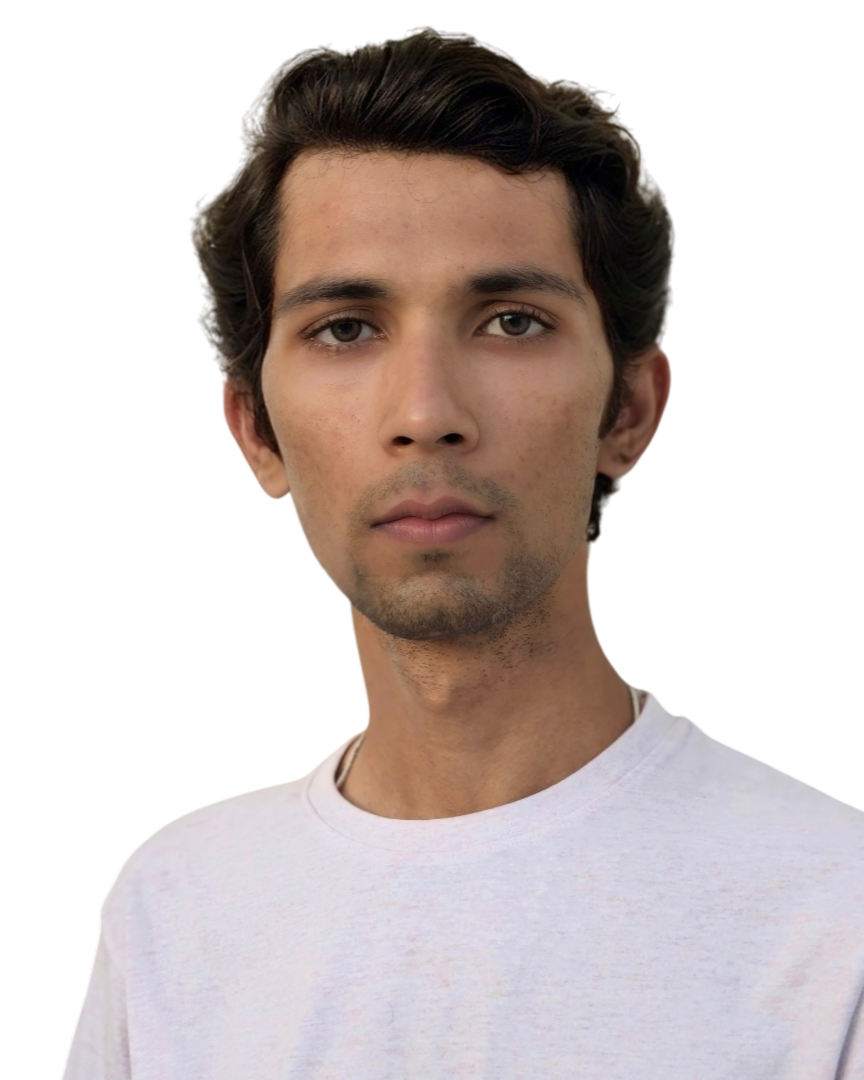
\includegraphics[width=3.6cm]{darshan_square.png}}
    \end{flushright}
\end{multicols}

\vspace{-2.5mm}
%-----------Technical skills-----------------
\section{\textbf{Profil}}

 \begin{itemize}[leftmargin=0.05in, label={}]
    \small\item {Full-Stack-Softwareentwickler mit mehr als 7 Jahren Erfahrung in der Entwicklung von Unternehmensanwendungen. Derzeit in Deutschland ansässig und im Masterstudium Software Engineering an der Hochschule Heilbronn. Spezialisiert auf die Modernisierung von Altsystemen, Leistungsoptimierung und Teamleitung in multikulturellen, verteilten Teams. Fundierte Kenntnisse in .NET, React und Azure-Cloud-Technologien, mit nachweislicher Erfahrung in der Stabilisierung von Altsystemen und der Reduzierung der Fehlererkennungszeit von Stunden auf Minuten. Fließend in Englisch mit ausbaufähigen Deutschkenntnissen, engagiert für eine langfristige Karriere in Deutschland.}
 \end{itemize}
 \vspace{-16pt}
%-----------EXPERIENCE-----------------
\section{\textbf{Berufserfahrung}}
\pagebreak[3]
  \resumeSubHeadingListStart
  \vspace{-1 mm}
    \pagebreak[2]
    \resumeSubheading
      {Reveation Labs}{Dez. 2022 - März 2025}
      {Softwareentwickler III (Full Stack)}{Remote, Indien}
      \vspace{-1.0mm}
      \resumeItemListStart
    \item {Entwarf ein Echtzeit-System zur Gesundheitsüberwachung mit React, Microservices, geplanten Aufgaben und Azure Workbooks. Dadurch wurden die Fehlererkennungszeiten von 8-10 Stunden auf 10-15 Minuten über mehr als 50 globale Anwendungen hinweg reduziert und die Reaktionsfähigkeit des Unternehmens verbessert.}
    \item {Stabilisierte ein altes Abonnementverwaltungssystem, das 50.000 Anbieter und 1 Million internationale Mitglieder bedient. Reduzierte Support-Tickets durch eine systematische Problemlösung um etwa 30 \% im Laufe des folgenden Jahres.}
    \item {Modernisierte Altsysteme durch Umstellung von TFS auf Git, Aktualisierung von Framework-Versionen und Implementierung automatisierter CI/CD-Pipelines für schnellere und zuverlässigere Bereitstellungen.}
    \item {Arbeitete mit Kollegen zusammen, um Microservices mit .NET 8, RabbitMQ und Web-APIs zu implementieren. Restrukturierte Legacy-Anwendungen, um die Verarbeitung von Mitgliederabonnements und die Systemskalierbarkeit zu verbessern.}
    \item {Leitete das Team während der PI-Planung, identifizierte wichtige Herausforderungen, schlug umsetzbare Lösungen vor und dokumentierte Strategien zur Verbesserung der Abstimmung und Effizienz zwischen Geschäfts- und IT-Teams; betreute dabei 4-5 Junior-Entwickler.}
    \item {Entwickelte neue Funktionen für ältere Windows-Anwendungen mit C\# und wartete gleichzeitig wichtige Funktionen in älteren VB-basierten Apps, um die Systemstabilität zu gewährleisten und die Benutzererfahrung zu verbessern.}
    \resumeItemListEnd
    
    \vspace{-3 mm}
    
    \pagebreak[2]
    \resumeSubheading
      {Tark Technologies LLP}{Dez. 2017 - Dez. 2022}
      {Junior Softwareentwickler, befördert zum Senior (2020)}{Rajkot, Indien}
      \vspace{-1.0mm}
      \resumeItemListStart
    \item {Entwickelte einen internen Alexa-Skill vollständig (Backend und Frontend) während der Sprachassistenten-Welle 2018 und verwaltete dessen Content-Pipeline.}
    \item {Modernisierte ein stark frequentiertes, mehrrollenfähiges POS-Portal von AngularJS über eine Hybridarchitektur zu Angular; verantwortete Backend-Services und Stored Procedures für 50.000 Bestellungen in den saisonalen Sommerspitzen.}
    \item {Baute ein ERP-System einer Reha-Einrichtung von klassischem ASP auf Angular um, modernisierte das Backend und verwaltete Aufnahme, Therapieplanung und Abrechnung gegenüber Partnerstiftungen für 300-400 gleichzeitige Patienten.}
    \item {Digitalisierte die papierbasierte Erfassung eines Gentestlabors mit einem React-Frontend über ein Multi-Stack-Backend und entwickelte die ETL-Pipeline für einen langfristigen Patientengesundheitsdatenspeicher über 150-180 Partnerkliniken.}
    \item {Befördert zum Senior im Jahr 2020; führte Code-Reviews und Pair-Programming-Sitzungen durch und coachte 4-5 Junior-Entwickler.}
    \resumeItemListEnd
    
    \vspace{-3.0mm}
    
  \resumeSubHeadingListEnd
\vspace{-8.5mm}

\vspace{2.5 mm}
%-----------PROJECTS-----------------
%-----------EDUCATION-----------
\section{\textbf{Bildungsweg}}
\pagebreak[3]
  \resumeSubHeadingListStart
  \vspace{-1 mm}
    \pagebreak[2]
    \resumeSubheading
      {Hochschule Heilbronn - Deutschland}{März 2025 - Heute}
      {Master of Science in Software Engineering and Management}{Heilbronn, Deutschland}
    \pagebreak[2]
    \resumeSubheading
      {Gujarat Technological University - Indien}{2013 - 2017}
      {Bachelor of Engineering in Informatik und Ingenieurwesen {\bf (CGPA - 8.24)}}{Ahmedabad, Indien}
  \resumeSubHeadingListEnd
\vspace{-5.5mm}

\section{\textbf{Technische Fähigkeiten}}
\pagebreak[3]
\begin{itemize}[leftmargin=0.05in, label={}]
    \small\item{
     \textbf{Programmierung}{: C\#, JavaScript, TypeScript, SQL, Python}\\
     \textbf{Frameworks}{: .NET, React.js, Angular, Entity Framework}\\
     \textbf{Datenbanken}{: SQL Server, MySQL, MongoDB}\\
     \textbf{Tools}{: Azure, Docker, Git, CI/CD, RabbitMQ}\\
     \textbf{Methoden}{: Agile/Scrum, Microservices}\\
     \textbf{Sprachen}{: Englisch (Fließend), Deutsch (A1), Hindi (Muttersprache), Gujarati (Muttersprache)} \\
    }
\end{itemize}
\vspace{-4.5 mm}
\vspace{0.5 mm}

\section{\textbf{Zertifizierungen}}
\pagebreak[3]
 \begin{itemize}[leftmargin=0.05in, label={}]
    \small\item{
     \textbf{Python 3 Programmierung}{: \href{https://coursera.org/share/ff34d909a15ffa2eec59e366533731b1}{Coursera}}
    }
 \end{itemize}
\vspace{-4.5mm}

\vspace{0.5 mm} % Adjust the vertical space as needed

\section{\textbf{Projekte}}
\pagebreak[3]
\resumeSubHeadingListStart
    \vspace{-1 mm}
     \pagebreak[2]
     \resumeProject
      {Persönliche Website \& stets aktueller Lebenslauf}{Design, Entwicklung, Automatisierung}{2025 - Heute}{\href{https://github.com/drshnmaniar/drshnmaniar.github.io}{github.com/drshnmaniar}}
      \resumeItemListStart
       \item {Entwickelte ein React-Portfolio mit allen Inhalten in einer einzigen JSON-Datei, sodass Textänderungen nie den Komponentencode berühren.}
       \item {Richtete eine GitHub-Actions-Pipeline ein, die den englischen und deutschen Lebenslauf bei jedem Push aus LaTeX kompiliert und die herunterladbaren PDFs stets aktuell hält.}
       \item {Open Source; das Repository dient zugleich als überprüfbare, praktische Arbeitsprobe.}
    \resumeItemListEnd
    \vspace{-2mm}

    \vspace{-1 mm}
     \pagebreak[2]
     \resumeProject
      {Akzeptanz von KI-Tools in der akademischen Forschung}{Studienprojekt (1. Semester)}{Apr. 2025 - Juli 2025}{Hochschule Heilbronn}
      \resumeItemListStart
       \item {Entwarf und implementierte eine strukturierte Umfragemethodik, die innerhalb von 29 Tagen 36 Antworten sammelte, um User-Experience-Muster und Adoptionsbarrieren für KI-Tools in Forschungsabläufen zu analysieren.}
       \item {Führte statistische Analysen und thematische Kodierungen quantitativer und Freitext-Daten mit deskriptiver Statistik und manuellen Analysetechniken durch.}
       \item {Stellte fest, dass 78 \% der Befragten Produktivitätssteigerungen berichteten, während Zuverlässigkeitslücken ihr Vertrauen in die Tools untergruben.}
       \item {Lieferte umsetzbare Erkenntnisse zu Tool-Fragmentierung, Preismodellen und Workflow-Optimierung, die in Empfehlungen für eine Plattformkonsolidierung einflossen.}
    \resumeItemListEnd
    \vspace{-2mm}

    \vspace{-1 mm}
    \pagebreak[2]
    \resumeProject
    {Modernisierung von Altsystemen \& DevOps Transformation}{Leitender Entwickler}{Dez. 2024 - Jan. 2025}{Reveation Labs}
    \resumeItemListStart
      \item {Leitete die Migration von Legacy-VB-Anwendungen von TFS zu Git, aktualisierte .NET-Framework-Versionen und modernisierte Entwicklungsabläufe für verbesserte Wartbarkeit.}
      \item {Entwarf eine modulare NuGet-Paketstrategie, die monolithische Legacy-Module in wiederverwendbare Komponenten umwandelte und Versionsinkonsistenzen über mehr als 200 Anwendungen hinweg beseitigte.}
      \item {Implementierte eine CI/CD-Pipeline mit automatisierten Code-Reviews und einer manuellen Testphase, wodurch die Bereitstellungszeit von 2-3 Stunden auf etwa 1 Stunde reduziert und konsistente Code-Qualitätsstandards in den Entwicklungsteams etabliert wurden.}
    \resumeItemListEnd
    \vspace{-2 mm}
    
    \vspace{-1 mm}
    \pagebreak[2]
    \resumeProject
      {Dashboard zur Systemüberwachung}{Senior Full-Stack-Entwickler}{Juni 2024 - Dez. 2024}{Reveation Labs}
         
      \resumeItemListStart
      \item {Entwarf eine umfassende Überwachungslösung für über 200 geschäftskritische Produktionssysteme, eliminierte das reaktive Störungsmanagement und stellte die Geschäftskontinuität sicher.}
      \item {Entwickelte ein Echtzeit-Dashboard mit intelligentem Alarmsystem, das die Mean Time to Detection (MTTD) von Stunden auf Minuten reduzierte und sich direkt auf die Kundenzufriedenheit auswirkte.}
      \item {Implementierte ein automatisiertes Benachrichtigungssystem mit kontextbezogener Fehleranalyse, was eine schnellere Identifizierung der Grundursache und eine proaktivere Störungsbehebung ermöglichte.}
      \item {Lieferte eine proaktive Überwachungslösung, die das Betriebsmodell von kundengemeldeten Problemen auf vorausschauende Wartung umstellte.}
      \item {Arbeitete mit funktionsübergreifenden Teams über mehrere Zeitzonen hinweg zusammen, um eine nahtlose Integration in die bestehende Unternehmensinfrastruktur sicherzustellen.}
      \resumeItemListEnd
    \vspace{-2 mm}
      
  \resumeSubHeadingListEnd
\vspace{-5.5mm}

\vspace{-1 mm}
\end{document}
